\section {Assignment 5 \\ {Convolution}}
\label {sec:assignment_5}

We wrote a convolutie 5x5 kernel with all 1's. The kernel put over the image from lab 2 is shown in figure \ref{fig:5x5}.

\begin{figure}[h!]
    \centering
    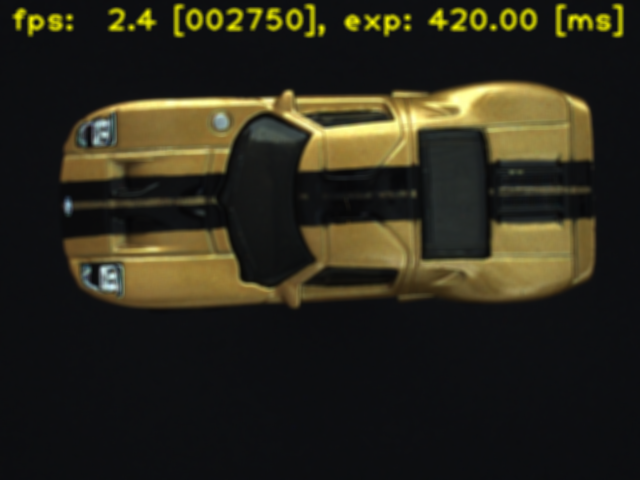
\includegraphics[width=0.45\textwidth]{5x5.png}
    \caption{5x5 kernel over image from lab 2}
    \label{fig:5x5}
\end{figure}

the code we used to make the kernel is shown in listing \ref{lst:5x5}.

\begin{lstlisting}[language=C, caption=5x5 kernel, label=lst:5x5]
void convolve5 (Mat* inputImg, Mat* outImg, int* kernel5){
    //I assume the mat is CV_8UC1 since I want to process BGR channels individually
    size s = inputImg->size();
    const uint8_t kernel_size = 5;
    uint8_t out[s.height][s.width];
    //int kernel[kernel_size][kernel_size] = {{1,1,1,1,1},{1,1,1,1,1},{1,1,1,1,1},{1,1,1,1,1},{1,1,1,1,1}};
    
    int x ,y, h, w, i, j, sum;
  
    for (h=0; h<s.height; h++){
        for(w=0; w<s.width; w++){
            sum = 0;
            for(i=0 ;i<kernel_size; i++ ){
                for(j=0; j<kernel_size; j++){
                    y=h-i+1; x=w-j+1;
                    if(y<0) y=0;
                    if(y>s.height-2) y=s.height-2;
                    if(x<0) x=0;
                    if(x>s.width-2) x=s.width-2;
                    //sum+=kernel[i][j]*inputImg->at<uint8_t>(y,x);
                    sum += *kernel5[i][j]*inputImg->at<uint8_t>(y,x);
                }
            }
            sum /= kernel_size*kernel_size;
            if(sum<0) sum=0;
            if(sum>255) sum=255;
            std::memcpy(outImg->data, out, s.height*s.width*sizeof(uint8_t));
        }
    }
}
\end{lstlisting}